%%% Template originaly created by Karol Kozioł (mail@karol-koziol.net) and modified for ShareLaTeX use

\documentclass[a4paper,11pt,pagenumber=true]{article}

\usepackage{graphicx,url}
\usepackage[brazil]{babel}   
\usepackage[utf8]{inputenc}  
\usepackage{dirtytalk}
\usepackage{verbatim}
\usepackage{listings}
\usepackage{xcolor}

%\renewcommand\familydefault{\sfdefault}
%\usepackage{tgheros}
%\usepackage[defaultmono]{droidmono}

\usepackage{pifont,textcomp,gensymb}
\usepackage{amsmath,amssymb,amsthm}
\usepackage{enumerate, multicol}
\usepackage{tikz, booktabs}

\usepackage{geometry}
\geometry{
    total={210mm,297mm},
    left=25mm,right=25mm,
    bindingoffset=0mm, 
    top=20mm,bottom=20mm
}
\linespread{1.3}

\newcommand{\linia}{\rule{\linewidth}{0.5pt}}

%% Shortcut macros.
%
% Vectors names:
\newcommand{\veca}{$\mathbf{a\,}$}
\newcommand{\vecr}{$\mathbf{r\,}$}
\newcommand{\vecn}{$\mathbf{n\,}$}
% Other math shortcuts (use only on math mode):
\newcommand{\vecnorm}[1]{\|\mathbf{#1}\|}
\newcommand{\dotprod}[2]{\mathbf{#1} \bullet \mathbf{#2}}
\renewcommand{\sin}{\text{\,sen\,}}
%%

\newtoks\institution

% custom theorems if needed
\newtheoremstyle{mytheor}
    {1ex}{1ex}{\normalfont}{0pt}{\scshape}{.}{1ex}
    {{\thmname{#1 }}{\thmnumber{#2}}{\thmnote{ (#3)}}}
\theoremstyle{mytheor}
\newtheorem{defi}{Definition}

% my own titles
\makeatletter
\renewcommand{\maketitle}{
    \begin{center}
        \vspace{2ex}
        {\huge \textsc{\@title}}
        \vspace{1ex}\\
        \linia\\
        \@author\\ 
        \linia\\
        \vspace{1ex}
        \textsc{\the\institution} 
        \hfill \@date
        \vspace{4ex}
    \end{center}
}
\makeatother
%%%

% custom footers and headers
\usepackage{fancyhdr}
\pagestyle{fancy}
\lhead{}
\chead{}
\rhead{}
\lfoot{Lista de Exercícios de Computação Gráfica \textnumero{3}}
\cfoot{}
\rfoot{Página \thepage}
\renewcommand{\headrulewidth}{0pt}
\renewcommand{\footrulewidth}{0pt}
%

% code listing settings
\usepackage{listings}
\renewcommand{\lstlistingname}{Listagem}
\renewcommand{\lstlistlistingname}{Relação de \lstlistingname s}
\lstset{
    language=Python,
    basicstyle=\ttfamily\small,
    aboveskip={1.0\baselineskip},
    belowskip={1.0\baselineskip},
    columns=fixed,
    extendedchars=true,
    breaklines=true,
    tabsize=4,
    prebreak=\raisebox{0ex}[0ex][0ex]{\ensuremath{\hookleftarrow}},
    frame=lines,
    showtabs=false,
    showspaces=false,
    showstringspaces=false,
    keywordstyle=\color[rgb]{0.627,0.126,0.941},
    commentstyle=\color[rgb]{0.133,0.545,0.133},
    stringstyle=\color[rgb]{01,0,0},
    numbers=left,
    numberstyle=\small,
    stepnumber=1,
    numbersep=10pt,
    captionpos=t,
    escapeinside={\%*}{*)},
    literate={á}{{\'a}}1 {â}{{\^a}}1 {ã}{{\~a}}1 {à}{{\`a}}1 {é}{{\'e}}1 {ê}{{\^e}}1 {ó}{{\'o}}1 {ô}{{\^o}}1 {õ}{{\~o}}1 {ú}{{\'u}}1 {~}{{\~}}1 {é}{{\'e}}1 {ç}{{\,c}}1 {í}{{\'i}}1
}

%%%----------%%%----------%%%----------%%%----------%%%

\begin{document}

    \title{Lista de Exercícios de\\Computação Gráfica \textnumero{3}}

    \author{Jonas de Araújo Luz Jr.\\
    unifor@jonasluz.com}
    \institution{Profa. Andreia Formico}
    \date{14/03/2017}
    
    % Unifor's logo
    \begin{figure}[t]
    \centering
        
\includegraphics[width=.2\textwidth]{images/logo-UNIFOR.jpg}
        \label{fig:logo}    
    \end{figure}
    %
    
    \maketitle
    \tableofcontents
    \newpage
    
    \section{Questão \textnumero{1}}
    
        Encontre o vetor reflexão \vecr, como mostra a figura abaixo, onde \vecn é o vetor normal. Sugestão: separe \veca em seus dois componentes vetoriais (vertical e horizontal).
        
        \begin{figure}[h]
            \centering
            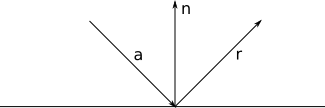
\includegraphics{images/Q-1.png}
            \label{fig:q1}
        \end{figure}
        
        \subsection*{Solução:}
        
            Dizer que \vecr é o vetor reflexão de \veca significa dizer que: 
            
            \begin{enumerate}
                \item A norma de \veca é igual à norma de \vecr, ou seja: $\vecnorm{a} = \vecnorm{r}$; e
                \item O ângulo $\alpha$ que \veca faz com o vetor normal \vecn é o mesmo que \vecr faz com o vetor normal \vecn.
            \end{enumerate}
            
            A partir disso, podemos verificar, geometricamente, conforme ilustra a Figura \ref{fig:q1a1}, que o ângulo $\beta$, diretor de \veca é o ângulo complementar de $\alpha$. 

            \begin{figure}[h]
                \centering
                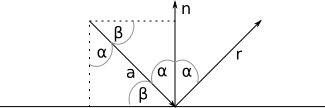
\includegraphics{images/Q-1-A-1.png}
                \caption{Identificando o ângulo $\beta$, diretor do vetor \veca.}
                \label{fig:q1a1}
            \end{figure}

            O vetor \veca pode ser escrito em função de seus componentes horizontal $\mathbf{a_x}$ e vertical $\mathbf{v_y}$:
            
            \begin{equation}
                \begin{matrix}
                    \mathbf{a} = \vecnorm{a} \cos \beta \mathbf{i} + \vecnorm{a} \sin \beta \mathbf{j} \\
                    \text{onde: } 
                        \mathbf{a_x} = \vecnorm{a} \cos \beta \mathbf{i} \text{ e } 
                        \mathbf{a_y} = \vecnorm{a} \sin \beta \mathbf{j}
                \end{matrix}
                \label{eq:a}
            \end{equation} 

            Alinhando as origens de todos os vetores, a Figura \ref{fig:q1a2} ilustra os vetores componentes de \veca. Verifica-se aí, geometricamente, que o ângulo $\theta$, diretor do vetor reflexão \vecr, corresponde ao ângulo diretor de \veca negado, ou seja: $\theta = -\beta$.
            
            \begin{figure}[h]
                \centering
                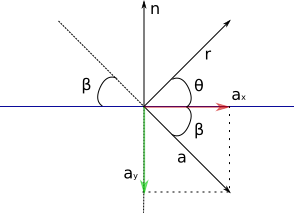
\includegraphics{images/Q-1-A-2.png}
                \caption{
                        Os vetores projeção de \veca, $\mathbf{a_x}$ e $\mathbf{a_y}$, e os ângulos diretores dos vetores \veca e \vecr, $\beta$ e $\theta$, respectivamente.  
                    }
                \label{fig:q1a2}
            \end{figure}

            Representando \vecr em função de seus vetores componentes $\mathbf{r_x}$ e $\mathbf{r_y}$, temos:
            
            \begin{equation}
                \begin{matrix}
                    \mathbf{r} = \vecnorm{r} \cos \theta \mathbf{i} + \vecnorm{r} \sin \theta \mathbf{j} \\
                    \text{onde: } 
                        \mathbf{r_x} = \vecnorm{r} \cos \theta \mathbf{i} \text{ e } 
                        \mathbf{r_y} = \vecnorm{r} \sin \theta \mathbf{j}
                \end{matrix}
                \label{eq:r}
            \end{equation}
            
            Sabendo que $\vecnorm{a} = \vecnorm{r}$ e colocando o valor de $\theta$ em função de $\beta$, obtemos, da Equação \ref{eq:r}:
            
            \begin{equation*}
                \begin{matrix}
                    \mathbf{r} = \vecnorm{a} \cos -\beta \mathbf{i} + \vecnorm{a} \sin -\beta \mathbf{j} 
                               = \vecnorm{a} \cos \beta \mathbf{i} - \vecnorm{a} \sin \beta \mathbf{j} \\
                    \text{onde: } 
                        \mathbf{r_x} = \vecnorm{a} \cos \beta \mathbf{i} \text{ e } 
                        \mathbf{r_y} = -\vecnorm{a} \sin \beta \mathbf{j} 
                \end{matrix} 
            \end{equation*}
            
            Disto, podemos, por fim, equacionar \vecr em função dos componentes horizontal e vertical de \veca, obtendo: 
            
            \begin{equation}
                \mathbf{r} = \mathbf{a_x} \mathbf{i} - \mathbf{a_y} \mathbf{j} 
                \label{eq:ra}
            \end{equation}

            A Figura \ref{fig:q1a3} ilustra os resultados encontrados.

            \begin{figure}[h]
            \centering
            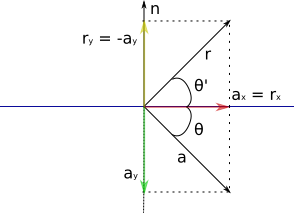
\includegraphics{images/Q-1-A-3.png}
                \caption{
                    Os vetores \veca e \vecr e seus componentes vetoriais 
                    $\mathbf{a_x}$, $\mathbf{a_y}$, $\mathbf{r_x}$ e $\mathbf{r_y}$
                }
                \label{fig:q1a3}
            \end{figure}

    \section{Questão \textnumero{2}}
    
        Suponha que você quer desfazer uma rotação de $\beta\degree$ (operação inversa) realizada no plano 2D. Utilizando uma matriz de rotação 2D genérica, deduza a nova matriz de rotação. Sugestão: rotacione de $-\beta\degree$ ou calcule a matriz transposta da rotação.

        \subsection*{Solução}
            
            A Figura \ref{fig:q2a} mostra um ponto $P(x, y)$ no plano 2D. O vetor do ponto $P$ é dado por $\mathbf{p}=\left<x, u\right>$ com ângulo diretor $\alpha$. Rotacionando-o em $\beta\degree$, obtém-se o ponto $P'(x', y')$, cujo vetor $\mathbf{p'}=\left<x', y'\right>$ possui ângulo diretor $\alpha + \beta$ e $\vecnorm{p'}=\vecnorm{p}$.
            
            \begin{figure}[h]
                \centering
                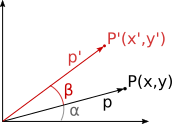
\includegraphics{images/Q-2-A.png}
                    \caption{Rotação do ponto $P$ em $\beta\degree$}
                    \label{fig:q2a}
            \end{figure}

            Disto, temos que:
            
            \begin{equation*}
                \begin{matrix}
                    x = \vecnorm{p}\cos\alpha \\
                    y = \vecnorm{p}\sin\alpha \\
                \end{matrix}
            \end{equation*}
            
            E daí: 
            
            \begin{equation}
                \begin{matrix}
                    \cos\alpha = \frac{x}{\vecnorm{p}} \\
                    \sin\alpha = \frac{y}{\vecnorm{p}} \\
                \end{matrix}
                \label{eq:p}
            \end{equation}

            Da Figura \ref{fig:q2a}, extraímos ainda:
            
            \begin{equation}
                \begin{matrix}
                    x' = \vecnorm{p}\cos(\alpha+\beta) \\
                    y' = \vecnorm{p}\sin(\alpha+\beta) \\
                \end{matrix}
                \label{eq:pr}
            \end{equation}

            Da trigonometria, sabe-se que:
            
            \begin{equation}
                \begin{matrix}
                    \sin(\alpha+\beta) = \sin\alpha\cos\beta + \sin\beta\cos\alpha \\
                    \cos(\alpha+\beta) = \cos\alpha\cos\beta - \sin\alpha\sin\beta \\
                \end{matrix}
                \label{eq:trig}
            \end{equation}
            
            Substituindo \ref{eq:trig} em \ref{eq:pr}, temos:
            
            \begin{equation}
                \begin{matrix}
                    x' = \vecnorm{p}\left(\cos\alpha\cos\beta - \sin\alpha\sin\beta\right) \\
                    y' = \vecnorm{p}\left(\sin\alpha\cos\beta + \sin\beta\cos\alpha\right) \\
                \end{matrix}
                \label{eq:rot}
            \end{equation}
            
            Substituindo \ref{eq:p} em \ref{eq:rot}, obtemos: 
            \[
                \begin{matrix}
                    x' = \vecnorm{p}\left(\frac{x}{\vecnorm{p}}\cos\beta - \frac{y}{\vecnorm{p}}\sin\beta\right) \\
                    y' = \vecnorm{p}\left(\frac{y}{\vecnorm{p}}\cos\beta + \frac{x}{\vecnorm{p}}\sin\beta\right) \\
                \end{matrix}
            \]

            Que resulta em: 
            \begin{equation}
                \begin{matrix}
                    x' = x\cos\beta - y\sin\beta \\
                    y' = x\sin\beta + y\cos\beta \\
                \end{matrix}
                \label{eq:frot}
            \end{equation}
            
            Escrevendo a Equação \ref{eq:frot} em forma matricial: 

            \begin{equation}
                \begin{bmatrix}
                    x' \\ y'
                \end{bmatrix} = 
                \begin{bmatrix}
                    \cos \beta & -\sin \beta  \\
                    \sin \beta & \cos \beta
                \end{bmatrix}
                \begin{bmatrix}
                    x \\ y
                \end{bmatrix}                
            \end{equation}

            Obtemos assim a matriz de rotação em $\beta\degree$ genérica no plano 2D, dada por: 
            
            \begin{equation}
                R = 
                \begin{bmatrix}
                    \cos \beta & -\sin \beta  \\
                    \sin \beta & \cos \beta
                \end{bmatrix}
                \label{eq:rotmatrix}
            \end{equation}
            
            Determinemos, agora, a matriz que resulta na operação inversa da rotação no plano 2D. Há duas formas de fazê-lo: 
            \begin{enumerate}
                \item Determinar a matriz transposta da matriz de rotação, dada em \ref{eq:rotmatrix}; e
                \item Efetuar a rotação de $P'$ em um ângulo igual a $-\beta\degree$, voltando ao ponto $P$.
            \end{enumerate}
            
            Tomemos o primeiro caso. \\
            
            Sabe-se que, dadas as matrizes $A$, $R$ e $A'$, tais que $R\bullet A=A'$, então a matriz transposta de $R$, dada por $R^T$, é tal que $R^T\bullet A' = A$.
            
            Disto, podemos concluir que a matriz transposta da matriz em \ref{eq:rotmatrix} $R^T$ é tal que: 
            \[
                R^T \bullet
                \begin{bmatrix}
                    x' \\ y'
                \end{bmatrix} = 
                \begin{bmatrix}
                    x \\ y
                \end{bmatrix}
            \]
            
            Pela definição da matriz transposta, temos que, para a matrix em \ref{eq:rotmatrix}: 
            
            \begin{equation}
                R^T = 
                \begin{bmatrix}
                    \cos\beta   && \sin\beta \\
                    -\sin\beta  && \cos\beta
                \end{bmatrix}
                \label{eq:rotinv}
            \end{equation}
            
            E esta é a matriz da operação inversa da rotação no plano 2D. \\
            
            Tomando o segundo caso, rotacionaremos $P'$ num ângulo de $-\beta\degree$. \\
            
            A matrix de rotação, neste caso fica:
            \[
                \begin{bmatrix}
                    \cos -\beta && -\sin -\beta  \\
                    \sin -\beta && \cos -\beta
                \end{bmatrix} = 
                \begin{bmatrix}
                    \cos\beta   && \sin\beta \\
                    -\sin\beta  && \cos\beta
                \end{bmatrix} = R^T \text{ dada em \ref{eq:rotinv}}
            \]
            
            E obtemos, assim também, a matriz $R^T$, da operação inversa da rotação no plano 2D.
            
    \section{Questão \textnumero{3}}

        Dada a figura abaixo, se $A_3$ é uma combinação convexa de $A_1$ e $A_2$, então qual a relação existente entre os vetores $A_3-A_2$ e $A_1-A_2$? 
        
        \begin{figure}[h]
        \centering
            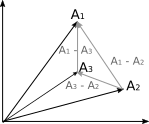
\includegraphics{images/Q-3.png}
            \label{fig:q3}
        \end{figure}        
        
        \subsection*{Solução}
        
            Por definição, se $A_3$ é uma combinação convexa de $A_1$ e $A_2$, então:
            
            \begin{equation}
                A_3 = a_1 A_1 + a_2 A_2 \text{ tal que: } a_1 + a_2 = 1 
                \text{, com } a_1 \geq 0 \text{ e } a_2 \geq 0 
            \end{equation}
            
            Podemos então escrever:
            \[
                A_3 - A_2 = a_1 A_1 + a_2 A_2 - A_2 = a_1 A_1 + (a_2 - 1) A_2 
                = a_1 A_1 - a_1 A_2 = a_1 (A_1 - A_2)
            \]
            
            Ou seja, a relação existente entre $A_3 - A_2$ e $A_1 - A_2$ é que o primeiro é uma combinação linear do segundo, sendo uma fração dele, tal que: 
            \begin{equation}
                A_3 - A_2 = a_1 (A_1 - A_2) \text{, com } 0 \leq a_1 \leq 1 
            \end{equation}
            
            Adicionalmente, é fácil verificar também que: 
            \[
                A_1 - A_3 = A_1 - (a_1 A_1 + a_2 A_2) = (1 - a_1) A_1 - a_2 A_2 
                = a_2 A_1 - a_2 A_2 = a_2 (A_1 - A_2)
            \]
            
            Ou seja, $A_1 - A_3$, também ilustrado na Figura \ref{fig:q3}, é, igualmente, uma combinação linear de $A_1 - A_2$. \\

            Com o que descobrimos, e sabendo que $a_1 + a_2 = 1$, podemos também \say{corrigir} o gráfico apresentado, que fica como mostrado na Figura \ref{fig:q3a}.
            
            \begin{figure}[h]
                \centering
                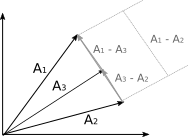
\includegraphics{images/Q-3-A.png}
                \caption{
                    Uma ilustração, mais próxima do real, das relações 
                    entre os vetores subtração de $A_1$, $A_2$ e $A_3$
                }
                \label{fig:q3a}
            \end{figure}
            
\nocite{*}
\bibliographystyle{acm}
\bibliography{assignment}

\end{document}
